\documentclass[11pt,a4paper,twoside,french,svgnames]{report}
\usepackage[utf8]{inputenc} % force the use of utf8
\usepackage[T1]{fontenc} % font encoding, allows accents
\usepackage[papersize={21cm,29.7cm},top= 2.5cm,bottom=2.5cm, inner=2.5cm, outer=2.5cm]{geometry} % page formatting
\usepackage[francais]{babel} % translate everything in the desired language: table of contents, etc. 'english' can be replaced with 'francais'
\usepackage{graphicx} % images management
\usepackage{wrapfig} % floating images
\usepackage{array} % allow arrays
\usepackage{fancyhdr} % headers/footers management (overrides empty, plain and headings)
\usepackage{listings} % code insertion (MUST BE WRITTEN AFTER BABEL)
%\usepackage[nottoc,numbib]{tocbibind} % bib in toc
%\usepackage{pdfpages} % include PDF documents
\usepackage{enumitem} % for /setlist
\usepackage{color,soul} % add some colors and hightlight
\usepackage{xcolor} % more colors
\usepackage[hyphens]{url} % auto break lines in URL
\usepackage{eurosym}
\usepackage{soulutf8}
\usepackage{color}
\usepackage{ulem}
\usepackage[babel=true]{csquotes}
\usepackage[hidelinks,  colorlinks  = true, % no borders, colors enabled
                        anchorcolor = blue,
                        linkcolor   = black, % links in table of contents
                        urlcolor    = blue,
                        citecolor   = blue]{hyperref}
%\usepackage[%nonumberlist,% no page number
%            toc,% displayed in toc
%            numberedsection,% displayed as a numbered section in toc
%            xindy]{glossaries} % glossary with xindy style. MUST BE WRITTEN AFTER HYPERREF
%\setglossarystyle{listgroup}

\sethlcolor{cyan} % package soul
\newcommand{\file}[1]{\hl{\emph{#1}}} % highlight a file URI

%\makeglossaries
%\loadglsentries{glossary.tex}

%%%%%%%%%%%%%%%%%%%%%%%%%%%%%%%%%%%%%%%%%%%%%%%%%%%%%%%% LISTINGS %%%%%%%%%%%%%%%%%%%%%%%%%%%%%%%%%%%%%%%%%%%%%%%%%%%%%%%%
\definecolor{comment}{rgb}{0.12, 0.38, 0.18 } % adjusted, in Eclipse: {0.25, 0.42, 0.30 } = #3F6A4D
\definecolor{keyword}{rgb}{0.37, 0.08, 0.25}  % #5F1441
\definecolor{string}{rgb}{0.06, 0.10, 0.98} % #101AF9

\lstset{
  columns=flexible, %prevent extra spaces
  rulecolor=\color{black!50},
  backgroundcolor = \color{blue!10},
  numbers=none, % line numbering
  showspaces=false,
  showtabs=false,
  breaklines=true,
  showstringspaces=false,
  breakatwhitespace=false,
  commentstyle=\color{comment},
  keywordstyle=\color{keyword},
  stringstyle=\color{string},
  basicstyle=\ttfamily,
  extendedchars=true,
  emph=[2]{In},
  emphstyle=[2]\color{black!70},
  morecomment=[l][\color{blue}]{Out},
  frame=single,
  frameround=tttt,
  framerule=0.3pt,
  framesep=4pt,
  belowcaptionskip=2.1pt,
  literate={à}{{\`a}}1 {â}{{\^a}}1 %                         letter a
           {À}{{\`A}}1 {Â}{{\^A}}1 %                         letter A
           {ç}{{\c{c}}}1 %                                   letter c
           {Ç}{{\c{C}}}1 %                                   letter C
           {é}{{\'e}}1 {è}{{\`e}}1 {ê}{{\^e}}1 {ë}{{\"e}}1 % letter e
           {É}{{\'E}}1 {È}{{\`E}}1 {Ê}{{\^E}}1 {Ë}{{\"E}}1 % letter E
           {î}{{\^i}}1 {ï}{{\"i}}1 %                         letter i
           {Î}{{\^I}}1 {Ï}{{\"I}}1 %                         letter I
           {ô}{{\^o}}1 %                                     letter o
           {Ô}{{\^O}}1 %                                     letter O
           {œ}{{\oe}}1 %                                     letter oe
           {Œ}{{\OE}}1 %                                     letter OE
           {ù}{{\`u}}1 {û}{{\^u}}1 {ü}{{\"u}}1 %             letter u
           {Ù}{{\`U}}1 {Û}{{\^U}}1 {Ü}{{\"U}}1 %             letter U
  % above is a hack to force UTF8 compatibility (only for french)
}

\newcommand{\textcode}[1]{\lstset{
  language=,
  title={{\setlength{\fboxsep}{1pt}\fcolorbox{orange}{yellow!20}{\sffamily\scriptsize
              \textcolor{gray!10}{\_}{#1}\textcolor{gray!10}{\_}}}}
  }
}

\newcommand{\vhdl}{\lstset{
  language=VHDL,
  title={{\setlength{\fboxsep}{1pt}\fcolorbox{orange}{yellow!20}{\sffamily\scriptsize
              \textcolor{gray!10}{\_}VHDL\textcolor{gray!10}{\_}}}}
  }
}
%%%%%%%%%%%%%%%%%%%%%%%%%%%%%%%%%%%%%%%%%%%%%%%%%%%%%%%%%%%%%%%%%%%%%%%%%%%%%%%%%%%%%%%%%%%%%%%%%%%%%%%%%%%%%%%%%%%%%%%%%%%

%\parindent=20pt
\fancypagestyle{plain}{
    % Headers
    \fancyhead[R]{Rapport IA02}
    \fancyhead[L]{Damien \textsc{MARIÉ} - Kyâne \textsc{PICHOU}}

    % Footers
    \renewcommand{\footrulewidth}{0.1pt}
    \fancyfoot[C]{Université de Technologie de Compiègne}
    \fancyfoot[LE]{\ifnum\thepage>0 \thepage \fi}
    \fancyfoot[RO]{\ifnum\thepage>0 \thepage \fi}
}

\fancypagestyle{empty}{%
    \renewcommand{\headrulewidth}{0pt} % No sub line
    \fancyhead{} % Empty the header

    \renewcommand{\footrulewidth}{0pt}
    \fancyfoot{}
}

\setlist[itemize,2]{label={$\bullet$}} % use bullets for nested itemize

% First page
\newcommand{\presentation}[1]{\vspace{0.3cm}\large{\textbf{#1}}\vspace{0.3cm}\\}
\newcommand{\presentationLarge}[1]{\vspace{0.3cm}\LARGE{\textbf{#1}}\vspace{0.3cm}\\}

% Overrides chapter (numbered and no-numbered) headings: remove space, display only the title
\makeatletter
  \def\@makechapterhead#1{%
  \vspace*{0\p@}% avant 50
  {\parindent \z@ \raggedright \normalfont
    %\ifnum \c@secnumdepth >\m@ne
    %    \huge\bfseries \@chapapp\space \thechapter
    %    \par\nobreak
    %    \vskip 20\p@
    %\fi
    \interlinepenalty\@M
    \Huge \bfseries \thechapter\quad #1
    \vskip 40\p@
  }}
  \def\@makeschapterhead#1{%
  \vspace*{0\p@}% before 50
  {\parindent \z@ \raggedright
    \normalfont
    \interlinepenalty\@M
    \Huge \bfseries  #1\par\nobreak
    \vskip 40\p@
  }}
\makeatother

\newcommand{\ignore}[1]{} % inline comments

\pagenumbering{arabic}
%\addtocounter{page}{-7} % page numbering starts at 1 + (-7)
\pagestyle{plain} % uses fancy

\title{Rapport IA02}
\author{Damien MARIÉ et Kyâne PICHOU}
\date\today

%\setcounter{tocdepth}{4}

\begin{document}
\thispagestyle{empty} % only for the current page

\begin{center}

\includegraphics[height=3cm]{UTC_logo.png}\\
\vspace{2.5cm}
\presentation{Université de Technologie de Compiègne}
\presentation{IA02}

\vspace{2cm}
\noindent\fbox{
\begin{minipage}{0.9\textwidth}
\begin{center}
    \presentationLarge{Rapport de TP}
    \presentationLarge{\Huge{Prolog Stock Exchange}}
\end{center}
\end{minipage}}
\vspace{3cm}

\presentation{Printemps 2015}
\vspace{1cm}

\def\arraystretch{1.5} % 1 is the default
\begin{tabular}{|>{\hfill\arraybackslash}p{5cm}|p{5cm}|}
\hline
    \multicolumn{2}{|c|}{Damien \textsc{MARIÉ} - Kyâne \textsc{PICHOU}}\\
\hline
    \multicolumn{2}{|c|}{\textit{\today}}\\% dates
\hline
\end{tabular}
\end{center}

\tableofcontents

\chapter{Introduction}
Dans le cadre des TP de l'UV IA02, nous devons implémenter une version Prolog du jeu Chicago Stock Exchange, un jeu de plateau sur le thème de la bourse et de la finance. A chaque tour, les joueurs déplacent un pion \enquote{trader} et récoltent 2 marchandises. Ils en gardent une et jettent l'autre, faisant évoluer la valeur des ces marchandises. Le but étant d'avoir le stock de marchandises ayant le plus de valeur à la fin du jeu.\\
\section{Structures de données}
\noindent Les différentes structures de données qui composent ce jeu seront implémentées sous forme de listes.
\paragraph{Bourse} La bourse est simplement une liste contenant 6 sous-listes (une par élément) formant un couple [marchandise,valeur].
\paragraph{Marchandises} Le jeu est composé de 9 piles de 4 marchandises (à l'état initial). Chaque pile forme une sous-liste de 4 éléments et ces sous-listes composent une grande liste représentant l'état de toutes les piles du jeu.
\paragraph{Trader} Le trader a une position qui est simplement représentée par le numéro de la pile où il se trouve.
\paragraph{Réserve}Le joueur accumule des ressources tout au long de la partie. Chaque jouer a donc une liste dédié contenant toutes les marchandies qu'il possède.
\paragraph{Coup de jeu}Lorsqu'un joueur joue, plusieurs paramètres sont à prendre en compte. Ces paramètres sont placés dans une liste contenant :
\begin{itemize}
	\item le joueur qui effectue l'action
    \item la valeur du déplacement effectué (1,2 ou 3)
    \item la ressource qui est conservée
    \item la ressource qui est jetée
\end{itemize}


\chapter{Principaux prédicats}
\section{Gestion du plateau}
\subsection{Affichage}
Pour l'affichage, le code est plutot simple. Nous avons même pu utiliser des codes ANSI afin de rendre le résultat attractif.
\begin{center}
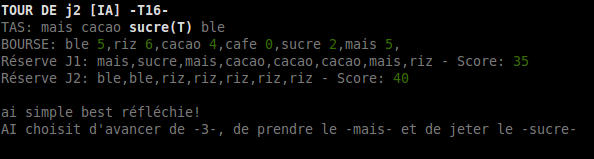
\includegraphics[height=3cm]{screen.png}\\
\end{center}
L'affichage inclut le score des joueurs et indique la position du trader sur les tas en plus des basiques.
\subsection{Génération du plateau}
En début de partie il faut générer les différentes structures qui composent un plateau. On crée donc un prédicat retournant un nouveau plateau.\\
Le prédicat va générer l'ensemble des piles en formant une liste, contenant des sous-listes de 4 éléments. Pour générer ces sous-listes, on tire un nombre au hasard, correspondant à l'indice d'un élément dans une grande liste contenant tout les jetons du jeu.
\begin{lstlisting}[language=prolog]
take_random(All,El,NewAll):-
	random_el(All,N),
	nth(N,All,El),
	select(El,All,NewAll)
\end{lstlisting}
Ensuite on génère la bourse, qui est toujours la même à l'état initial. On récupère donc simplement une liste hardcodée correspondant à l'état initial de la bourse.\\
De plus on génère un chiffre entre 1 et 9 correspondant à la position du trader.

\section{Déroulement du jeu}
\subsection{Vérification de coup}
Il est important de vérifier qu'un coup respecte les règles du jeu lorsqu'il est executé. Pour cela on utilise un prédicat \textit{coup\_possible} qui va prendre en entrée un plateau de jeu et qui va vérifier que le coup proposé est valide. \\
On commence par tester que la valeur du déplacement est bien de 1, 2 ou 3. Puis on effectue réellement le déplacement afin de récupérer la nouvelle position du trader. A partir de la nouvelle position du trader, on en déduit les éléments se trouvant sur le dessus des piles adjacentes. Enfin, on vérifie que les éléments à jeter et garder correspondent bien à ceux présents sur le haut des piles.\\
Concernant le déplacement du trader, on additionne simplement sa position avec le valeur du déplacement. On prend cependant garde à ne pas dépasser le nombre de pile, si c'est la cas alors on effectue un bouclage pour revenir au début du plateau.\\
Pour la vérification des éléments, on appelle un prédicat \textit{choix} qui va retourner les 2 éléments disponibles en fonction de la position du trader. Ce prédicat récupère le nombre de pile puis la position des piles autour du trader. Puis il récupère simplement les éléments en haut des piles corespondantes.

\section{Intelligence artificielle}
Nous avons programmé plusieurs intelligences artificielles afin de pouvoir avoir un benchmark de celles-ci:
\begin{itemize}
    \item Une intelligence purement aléatoire, qui choisit un coup aléatoire parmis les coups possibles (\textit{ai\_random})
    \item Une intelligence qui regarde à un seul niveau les scores possibles (\textit{ai\_simple\_best})
    \item Une intelligence qui utilise l'algorithme minimax (\textit{ai\_minimax})
\end{itemize}

Pour l'intelligence minimax, le seul problème est que la profondeur est limitée à 3 si l'on ne veut pas trop avoir de stackoverflow et à 2 si l'on veut pouvoir faire une partie complète.
Nous avons aussi programmé des combats entre ces IA afin de tester leurs performances, voici les résultats de pourcentages de vainqueurs selon les IAs:

\begin{lstlisting}
Random VS Random
j1 :73.5%
j2 :20.0%
j1 et j2 :6.5%

Random vs Simple best
j2 :94.0%
j1 :4.5%
j1 et j2 :1.5%

Simple best vs Random
j1 :97.5%
j1 et j2 :2.0%
j2 :0.5%

Simple best vs Simple best
j1 :67.0%
j2 :27.5%
j1 et j2 :5.5%

Depth 3 vs Depth 3
j1 :72.9%
j2 :25.7%
j1 et j2 :1.4%
\end{lstlisting}

On voit bien qu'une intelligence de profondeur 1 est déja trés efficace par rapport à un jeu aléatoire. On peut donc facilement imaginer les gains d'une IA de profondeur supérieure.\\
On remarque que le joueur 1 à un avantage stratégique évident (70\% de chance de gagner à coups alétoires, 67\% dans le cas de coups moins aléatoires).\\

\chapter{Conclusion}
Nous avons bien réussi à implémenter une version Prolog du jeu Chicago Exchange. Le jeu est complet, c'est à dire qu'il se déroule correctement et répond au cahier des charges :
\begin{itemize}
   \item Partie Humain vs Humain
   \item Partie IA vs Humain
   \item Partie IA vs IA
\end{itemize}
Prolog était un language trés adapté pour ce probléme. L'implémentation \textit{gprolog} n'est peut être pas assez évoluée, outillée et documentée pour permettre un dévelopement confortable mais celà ne nous à pas empécher à déveloper des fonctionnalités avancées.\\
Entre autre la gestion des marchandises, de la bourse, des réserves et de la position du trader sont implémentés, fonctionnels et sans failles. Notre intelligence artificielle reste cependant rudimentaire, c'est à dire qu'elle n'implémente pas l'algorithme \textit{minimax} et ne fait ses calculs que en fonction de l'état courant du plateau. Dans un sens, cette technique est la plus logique étant donné que les joueurs ne peuvent savoir que la marchandise se trouvant sur le dessus de la pile, regarder en dessus et donc calculer les prochains états du jeu relève donc de la triche.\\
Néanmoins nous avons essayé d'implémenter l'algorithme \textit{minimax}, mais celui-ci ne fonctionne qu'avec une profondeur de 1. Notre implémentation n'était donc pas opérationnelle, nous avons conservé notre IA basique.
\end{document}
